\documentclass{article}
\usepackage[utf8]{inputenc}
\usepackage{subfiles} 
\usepackage{fancyhdr}
\usepackage{graphicx}

\title{DevOps projectreport \\[2ex] 
\includegraphics[scale=0.1]{images/ITU_logo_UK.jpg}}
\author{Joachim Køcher Kelsen (jokk@itu.dk) \and Victor Nordestgaard (vino@itu.dk) \and Isabella Drest Rasmussen (iras@itu.dk) \and Anne Siemkowicz (asie@itu.dk) \and Bjørnar Haugstad Jåtten(bjja@itu.dk)}
\date{19 May 2021}

\usepackage{geometry}
\geometry{
 a4paper,
 total={210mm,297mm},
 left=30mm,
 right=30mm,
 top=25mm,
 bottom=20mm,
 }

\pagestyle{fancy}
\fancyhf{}
\rhead{Pythonkindergarten/Group J}
\lhead{DevOps projectreport}
\rfoot{Page \thepage}

\begin{document}{}

\maketitle

\newpage

\tableofcontents

\newpage

\subfile{sections/introduction.tex}

\newpage

\subfile{sections/LessonsLearnedPerspective.tex}

\newpage

\subfile{sections/ProcessPerspective.tex}

\newpage

\subfile{sections/SystemsPerspective.tex}

\newpage

\section{References}
\begin{thebibliography}{9}
\bibitem{devopshandbook} 
Stefan Thorpe.
\textit{DevOps Handbook Series Part 1: The Three Ways}. 
10.23.2017
\begin{verbatim}
https://caylent.com/devops-handbook-part-1-the-three-ways-2
\end{verbatim}

\bibitem{lecture02} 
Helge Pfeiffer. 
\textit{Session 02: Version control systems (Git), branching strategies, and collaborative development workflows}. 
\begin{verbatim}
https://github.com/itu-devops/lecture_notes/blob/master/sessions/session_02
\end{verbatim}

\bibitem{prometheusnet}
prometheus-net. \textit{prometheus-net}. 2021
\begin{verbatim}
https://github.com/prometheus-net/prometheus-net
\end{verbatim}

\bibitem{prometheusdotnetmetrics}
Djluck. \textit{prometheus-net.DotNetMetrics}. 2021
\begin{verbatim}
https://github.com/djluck/prometheus-net.DotNetRuntime
\end{verbatim}

\bibitem{prometheusaspnet}
Rocklan. \textit{prometheus-net.AspNet}. 2021
\begin{verbatim}
https://github.com/rocklan/prometheus-net.AspNet
\end{verbatim}

\bibitem{GitBranching} 
Scott Chacon. \textit{3.4 Git Branching - Branching Workflows}. 2021
\begin{verbatim}
https://git-scm.com/book/en/v2/Git-Branching-Branching-Workflows#_topic_branch
\end{verbatim}

\end{thebibliography}

\newpage

\section{Appendix}
\begin{figure}[h!]
    \centering
    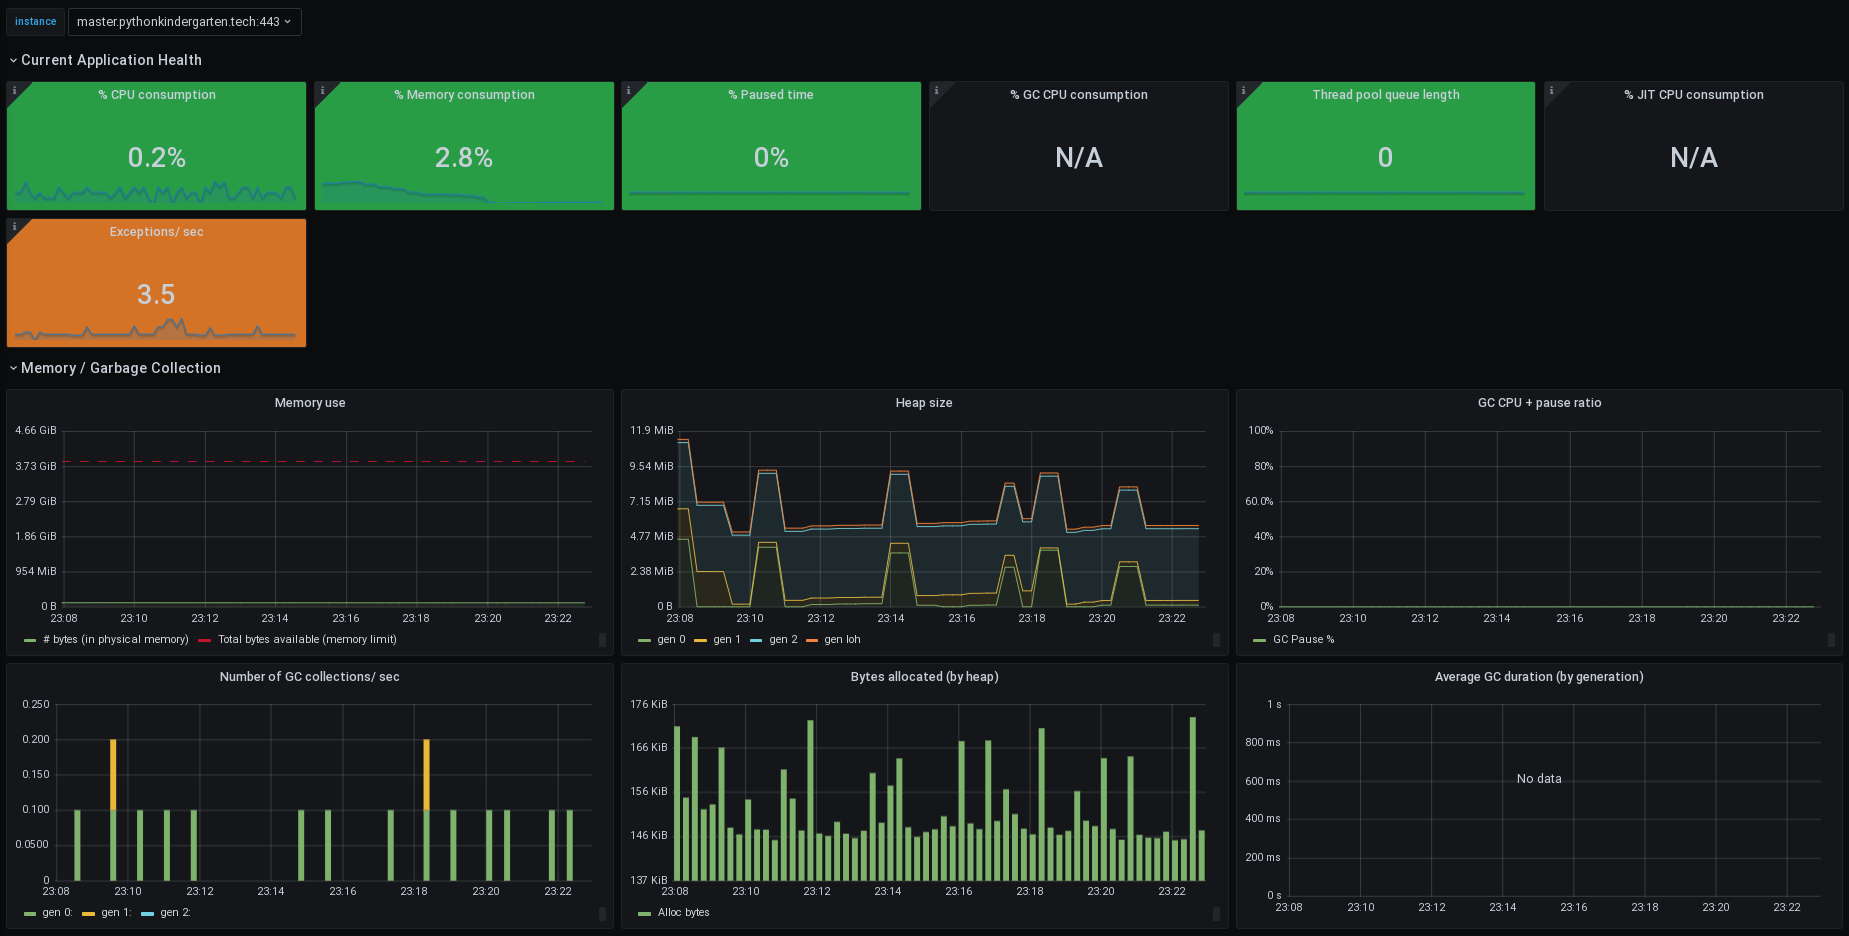
\includegraphics[scale=0.2]{images/grafana_1.png}
    \caption{ Our graphs in Grafana }
\end{figure}

\begin{figure}[h!]
    \centering
    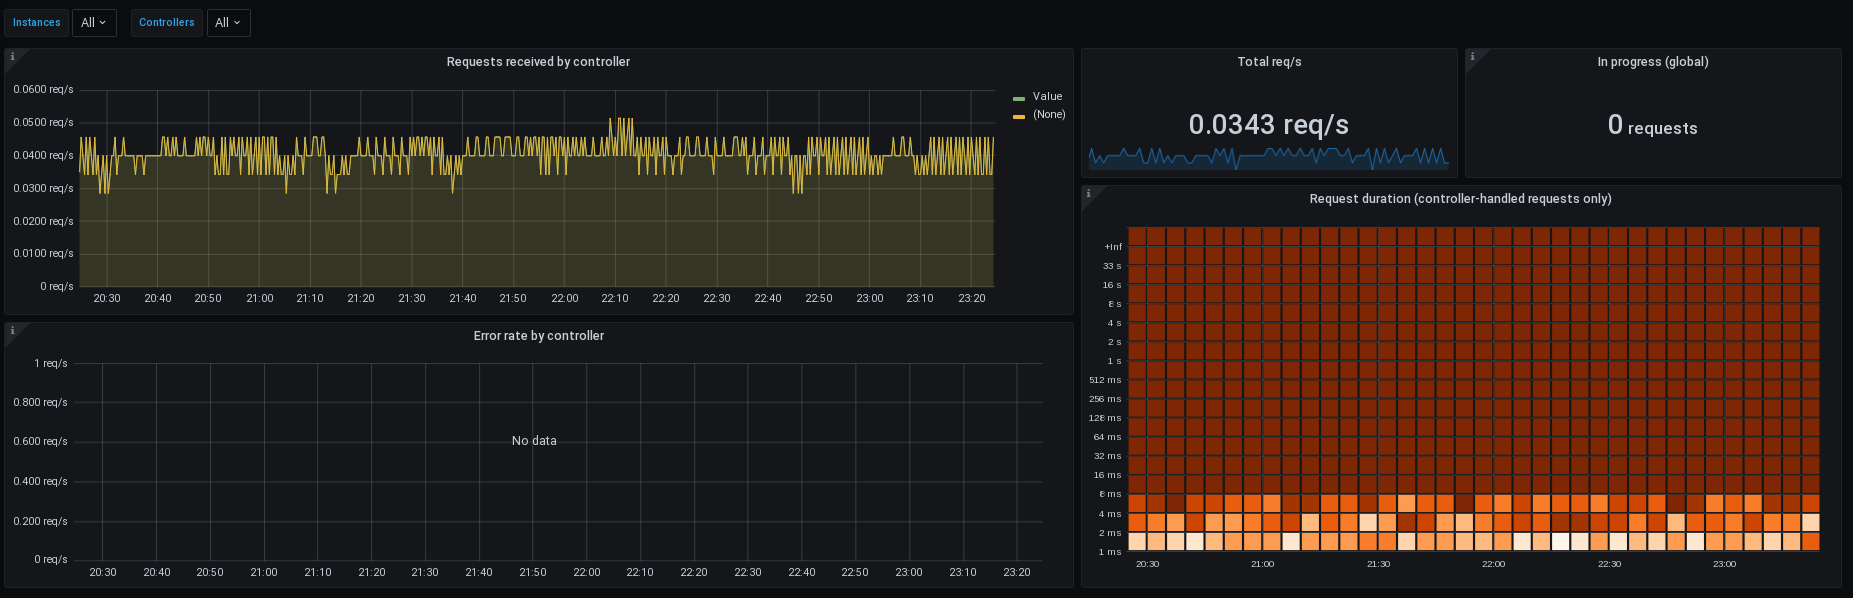
\includegraphics[scale=0.2]{images/grafana_2.png}
    \caption{ Our graphs in Grafana }
\end{figure}

\begin{figure}[h!]
    \centering
    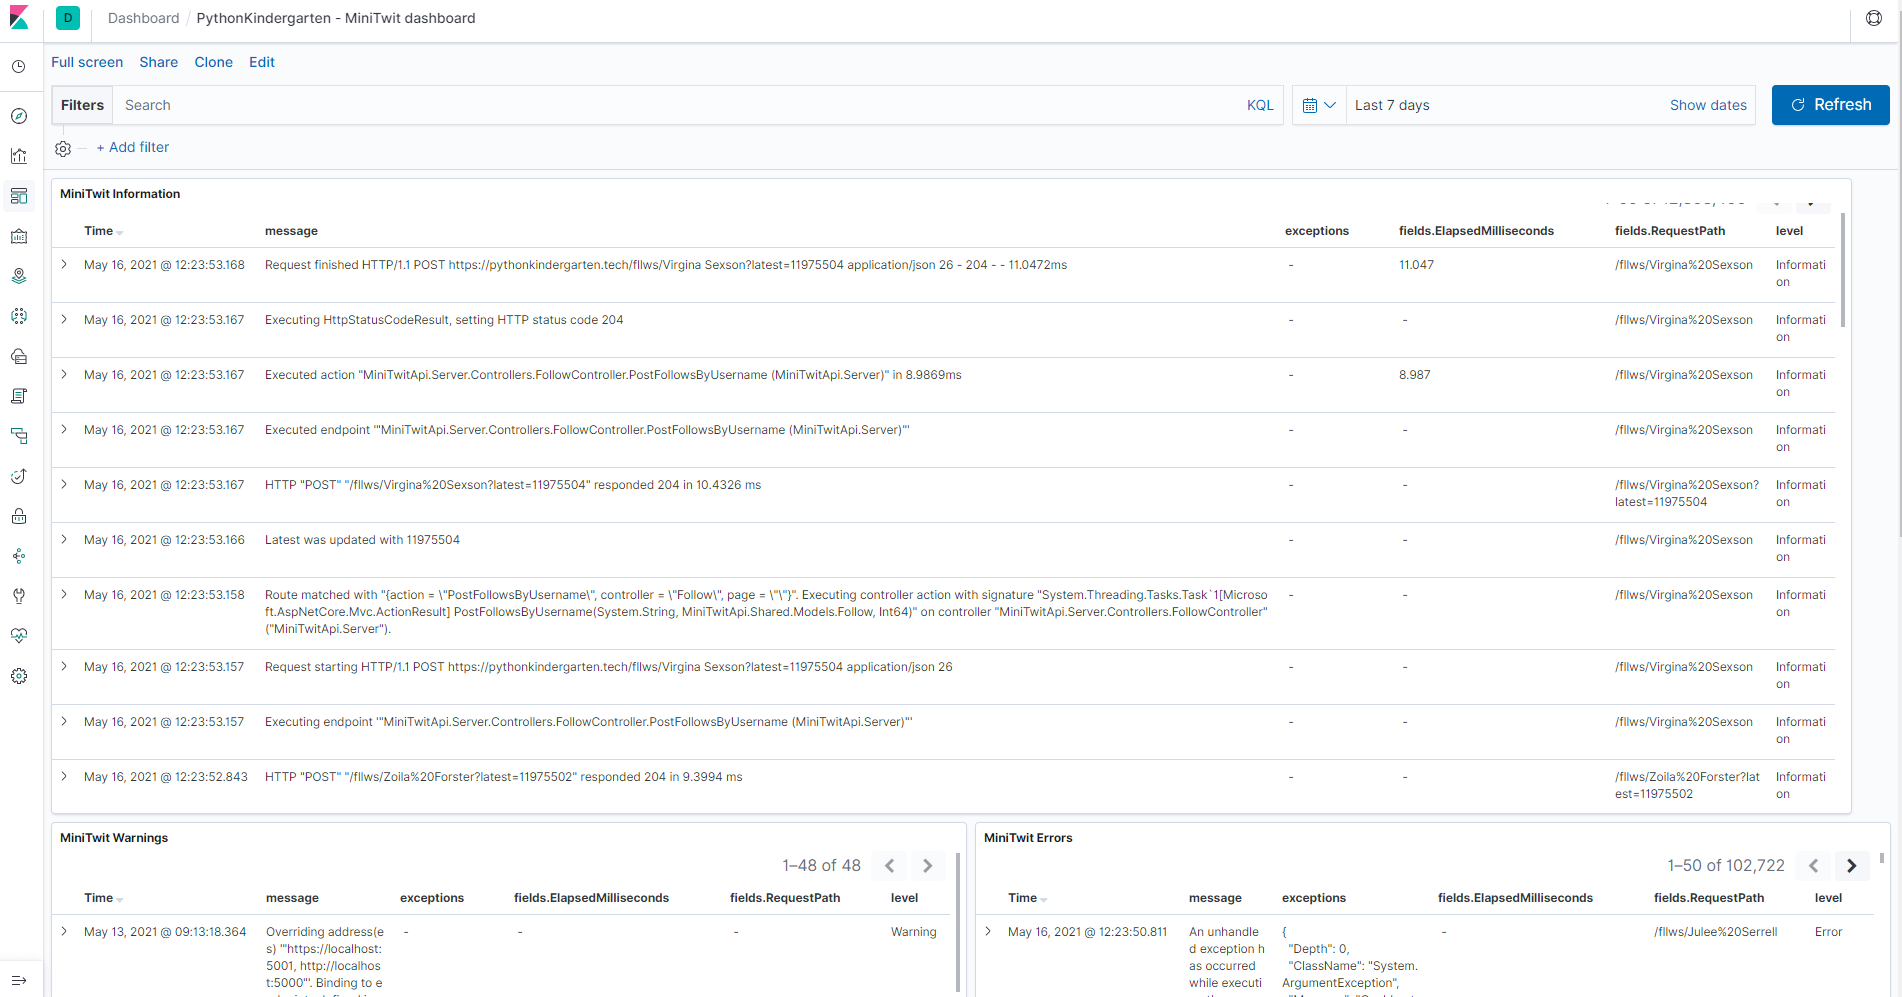
\includegraphics[scale=0.2]{images/kibana_1.png}
    \caption{ Current setup in Kibana }
\end{figure}

\begin{figure}[h!]
    \centering
    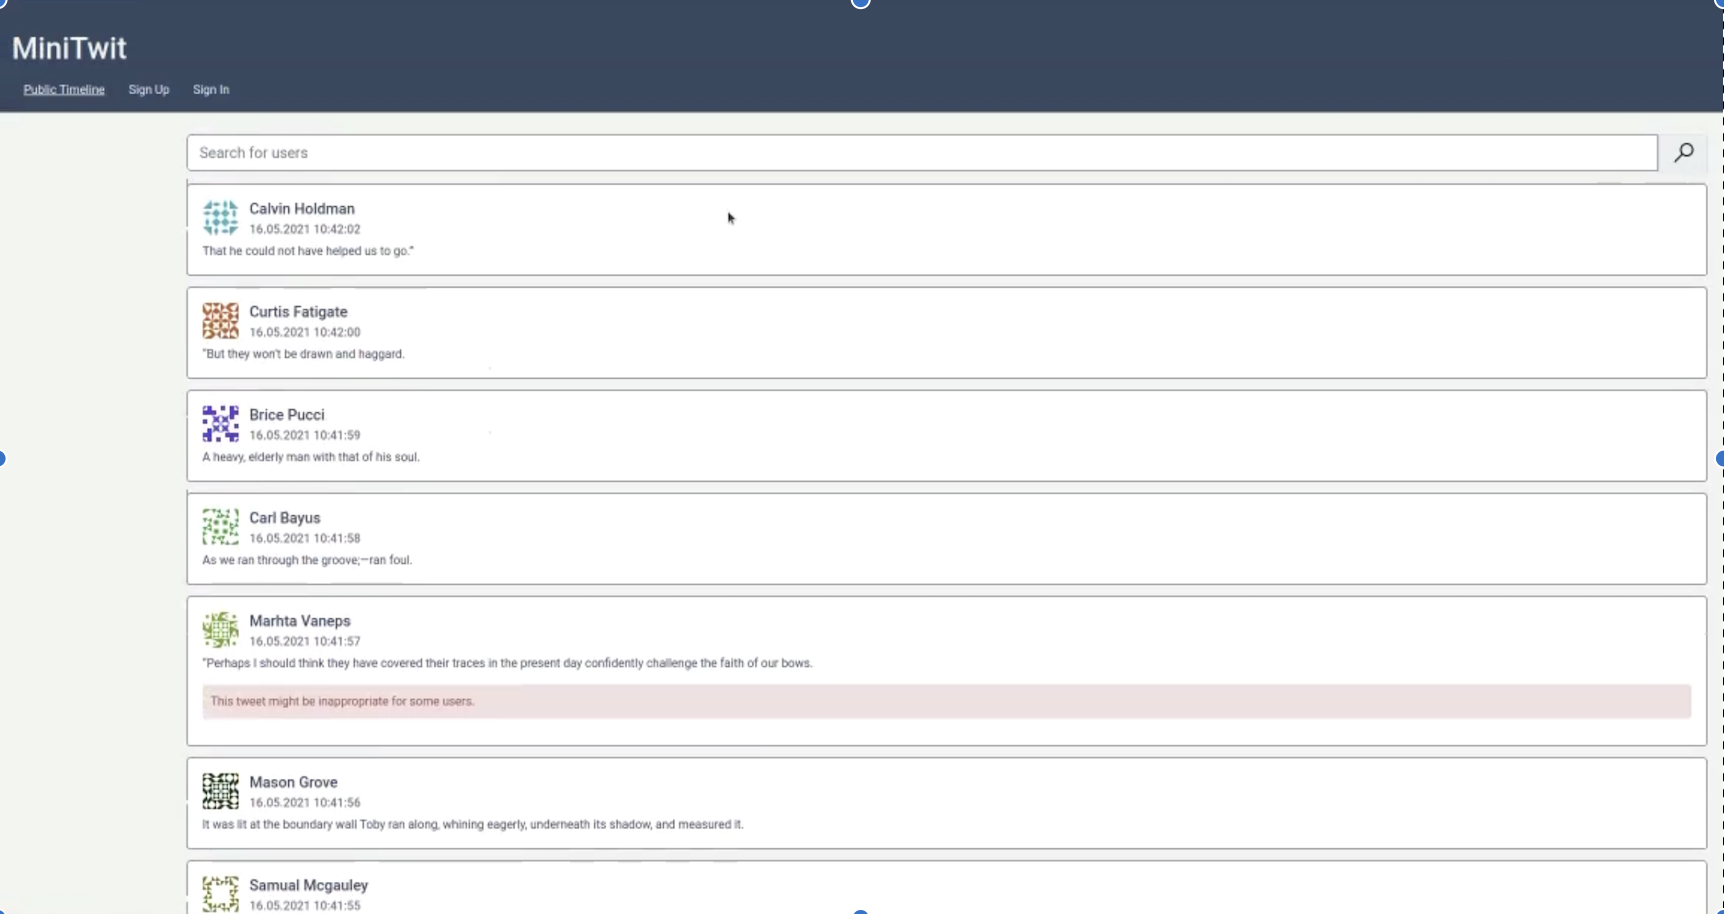
\includegraphics[scale=0.5]{images/minitwit.png}
    \caption{ Current look in our MiniTwit App }
\end{figure}

\newpage
\subsubsection{Security Assessment: Risk Matrixes}
\begin{figure}[h!]
    \centering
    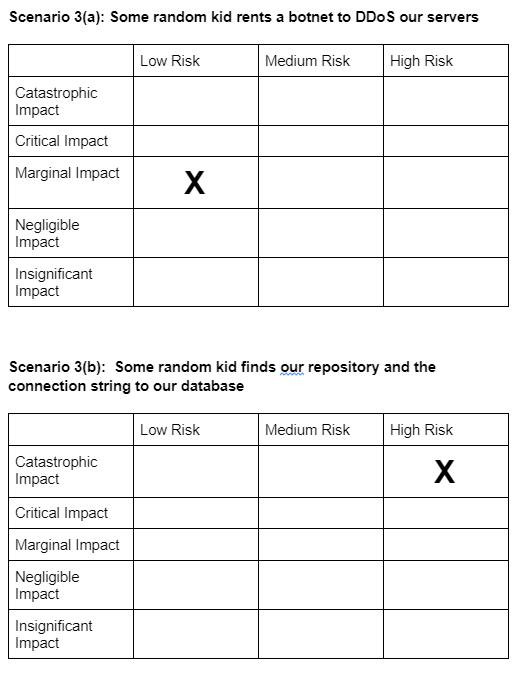
\includegraphics[scale=0.5]{images/risk_1.PNG}
    \caption{ Scenario 3a and 3b }
\end{figure}

\begin{figure}[h!]
    \centering
    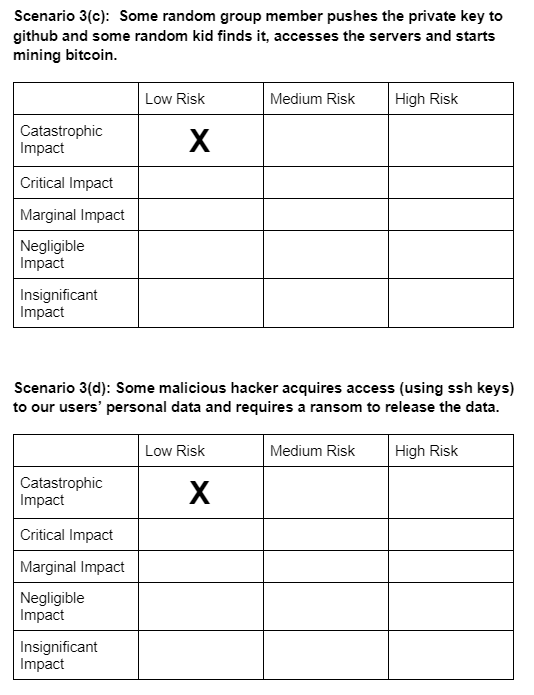
\includegraphics[scale=0.5]{images/risk_2.PNG}
    \caption{ Scenario 3c and 3d }
\end{figure}

\begin{figure}[h!]
    \centering
    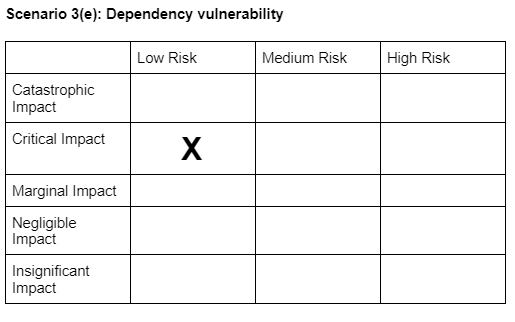
\includegraphics[scale=0.5]{images/risk_3.PNG}
    \caption{ Scenario 3e }
\end{figure}

\newpage
\subsection{Artifact Links}
Due to a late automation of system deployment in connection with the setup of Terraform, the logging and monitoring 
subsystems are not currently configured, as they once were earlier on in the project. We are at the time of writing working on reconfiguring these systems.

\textbf{Our MiniTwit application}
\begin{verbatim}
    https://pythonkindergarten.tech/
\end{verbatim}

\textbf{API MiniTwit}
\begin{verbatim}
    https://api.pythonkindergarten.tech/
\end{verbatim}

\textbf{Database}
\begin{verbatim}
    https://db.pythonkindergarten.tech/
\end{verbatim}

\textbf{Master/Slave}
\begin{verbatim}
    https://master.pythonkindergarten.tech/
    https://slave.pythonkindergarten.tech/
\end{verbatim}

\textbf{Monitoring}
\begin{verbatim}
    https://monitoring.pythonkindergarten.tech/
\end{verbatim}

\textbf{Logging}
\begin{verbatim}
    https://logging.pythonkindergarten.tech/
\end{verbatim}

\textbf{Repository}
\begin{verbatim}
https://github.com/jokk-itu/PythonKindergarten
\end{verbatim}

\textbf{Issue tracker}
\begin{verbatim}
https://github.com/jokk-itu/PythonKindergarten/issues
\end{verbatim}

\textbf{Wiki}
\begin{verbatim}
https://github.com/jokk-itu/PythonKindergarten/wiki
\end{verbatim}

\textbf{Project/Kanban-board}
\begin{verbatim}
https://github.com/jokk-itu/PythonKindergarten/projects/3
\end{verbatim}

\end{document}
